\documentclass[preview]{standalone}

\usepackage{amsmath}
\usepackage{amssymb}
\usepackage{stellar}
\usepackage{definitions}
\usepackage{bettelini}
\usepackage{tikz}

\begin{document}

\id{linearalgebra-coordinatized-vectors}
\genpage

\section{Coordinate vectors}

\begin{snippetdefinition}{cartesian-plane-definition}{Cartesian plane}
    The \emph{Cartesian plane} is the \set
    \[
        \realnumbers^2
        =
        \realnumbers \cartesianprod \realnumbers
        =
        \{(x,y) \suchthat x,y\in\realnumbers\}.
    \]
    The numbers \(x\) and \(y\) are called the \emph{coordinates} of the
    point \((x,y)\). The point \(O=(0,0)\) is called the \emph{origin}.
\end{snippetdefinition}

\begin{snippet}{point-as-coordinate-vector}
    Once the origin \(O=(0,0)\) has been fixed, a point
    \(P=(x,y)\in\realnumbers^2\) can be represented by the \vector
    \[
        \overrightarrow{OP}=(x,y).
    \]
    For example, if \(P=(3,2)\), then
    \[
        \overrightarrow{OP}=(3,2).
    \]
    \[
        \begin{tikzpicture}[scale=0.75]
            \draw[->] (-0.4,0)--(4,0) node[right] {\(x\)};
            \draw[->] (0,-0.4)--(0,3) node[above] {\(y\)};
            \fill (0,0) circle (1.5pt) node[below left] {\(O\)};
            \draw[->] (0,0)--(3,2);
            \fill (3,2) circle (1.5pt) node[above right] {\(P=(3,2)\)};
        \end{tikzpicture}
    \]
\end{snippet}

\begin{snippetdefinition}{coordinate-vector-addition-definition}{Addition of coordinate vectors}
    Let
    \[
        u=(x_1,y_1),
        \qquad
        v=(x_2,y_2)
    \]
    be two \vector[vectors] in \(\realnumbers^2\). Their sum is defined componentwise by
    \[
        u+v=(x_1+x_2,y_1+y_2).
    \]
\end{snippetdefinition}

\begin{snippet}{coordinate-vector-addition-geometry}
    The sum of two \vector[vectors] in \(\realnumbers^2\) can be visualized by the
    parallelogram rule:
    \[
        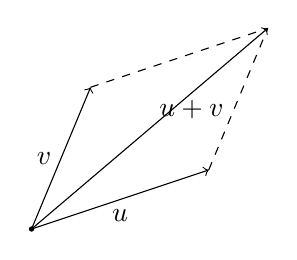
\begin{tikzpicture}[scale=0.75]
            \coordinate (O) at (0,0);
            \coordinate (U) at (3,1);
            \coordinate (V) at (1,2.4);
            \coordinate (S) at (4,3.4);

            \draw[->] (O)--(U) node[midway, below] {\(u\)};
            \draw[->] (O)--(V) node[midway, left] {\(v\)};
            \draw[dashed] (U)--(S);
            \draw[dashed] (V)--(S);
            \draw[->] (O)--(S) node[midway, above right] {\(u+v\)};
            \fill (O) circle (1.3pt);
        \end{tikzpicture}
    \]
\end{snippet}

\begin{snippetdefinition}{coordinate-vector-scalar-multiplication-definition}{Scalar multiplication of coordinate vectors}
    Let \(v=(x,y)\in\realnumbers^2\) and let
    \(\lambda\in\realnumbers\). The scalar multiple of \(v\) by \(\lambda\)
    is
    \[
        \lambda v=\lambda(x,y)=(\lambda x,\lambda y).
    \]
\end{snippetdefinition}

\begin{snippet}{coordinate-vector-scalar-multiplication-geometry}
    Let \(v\in\realnumbers^2\) and \(\lambda\in\realnumbers\).
    Geometrically, \(\lambda v\) has the same direction as \(v\) if
    \(\lambda>0\), the opposite direction if \(\lambda<0\), and is the zero
    \vector if \(\lambda=0\).
\end{snippet}

\begin{snippetproposition}{r2-vector-space-example}{The coordinate plane as a vector space}
    The \set \(\realnumbers^2\), with componentwise vector addition and scalar
    multiplication by real numbers, is a \vectorspace over \(\realnumbers\).
\end{snippetproposition}

\begin{snippetproof}{r2-vector-space-example-proof}{r2-vector-space-example}{The coordinate plane as a vector space}
    The zero \vector is \((0,0)\), and the additive inverse of
    \((x,y)\in\realnumbers^2\) is \((-x,-y)\). Associativity, commutativity of
    addition, and the distributive laws follow componentwise from the
    corresponding properties of real numbers. Therefore \(\realnumbers^2\) is
    a \vectorspace over \(\realnumbers\).
\end{snippetproof}

\section{Dot product}

\begin{snippetdefinition}{dot-product-r2-definition}{Dot product on the coordinate plane}
    Let
    \[
        u=(x_1,y_1),
        \qquad
        v=(x_2,y_2)
    \]
    be two \vector[vectors] in \(\realnumbers^2\). The \emph{dot product} of \(u\) and
    \(v\) is the real number
    \[
        u\cdot v=x_1x_2+y_1y_2.
    \]
\end{snippetdefinition}

\begin{snippetdefinition}{coordinate-vector-norm-r2-definition}{Norm in the coordinate plane}
    Let \(v=(x,y)\in\realnumbers^2\). The \emph{Euclidean norm} of \(v\) is
    \[
        \|v\|=\sqrt{x^2+y^2}.
    \]
    Equivalently,
    \[
        v\cdot v=\|v\|^2.
    \]
\end{snippetdefinition}

\begin{snippetdefinition}{coordinate-vector-orthogonality-r2-definition}{Orthogonality in the coordinate plane}
    Let \(u,v\in\realnumbers^2\). The \vector[vectors] \(u\) and \(v\) are
    \emph{orthogonal} if
    \[
        u\cdot v=0.
    \]
\end{snippetdefinition}

\begin{snippetexample}{coordinate-vector-orthogonality-example}{Orthogonal coordinate vectors}
    In \(\realnumbers^2\), the \vector[vectors] \((1,0)\) and \((0,1)\) are
    orthogonal because
    \[
        (1,0)\cdot(0,1)=1\cdot 0+0\cdot 1=0.
    \]
    Moreover,
    \[
        \|(1,0)\|=\sqrt{1^2+0^2}=1.
    \]
\end{snippetexample}

\section{Higher dimensions}

\begin{snippetdefinition}{coordinate-space-rn-definition}{Coordinate space}
    Let \(n\in\naturalnumbers\). The real coordinate space of \lineardimtext \(n\)
    is
    \[
        \realnumbers^n
        =
        \{(x_1,\ldots,x_n)\suchthat x_i\in\realnumbers
        \text{ for every } i=1,\ldots,n\}.
    \]
    Vector addition and scalar multiplication are defined componentwise:
    \[
        (x_1,\ldots,x_n)+(y_1,\ldots,y_n)
        =
        (x_1+y_1,\ldots,x_n+y_n),
    \]
    \[
        \lambda(x_1,\ldots,x_n)
        =
        (\lambda x_1,\ldots,\lambda x_n).
    \]
    The zero \vector is \(0=(0,\ldots,0)\).
\end{snippetdefinition}

\begin{snippetdefinition}{dot-product-rn-definition}{Dot product on real coordinate space}
    Let
    \[
        x=(x_1,\ldots,x_n),
        \qquad
        y=(y_1,\ldots,y_n)
    \]
    be \vector[vectors] in \(\realnumbers^n\). Their \emph{dot product} is
    \[
        x\cdot y=\sum_{i=1}^n x_i y_i.
    \]
\end{snippetdefinition}

\begin{snippetdefinition}{coordinate-vector-norm-rn-definition}{Norm in real coordinate space}
    Let \(x=(x_1,\ldots,x_n)\in\realnumbers^n\). The Euclidean norm of \(x\)
    is
    \[
        \|x\|=\sqrt{x\cdot x}
        =
        \sqrt{\sum_{i=1}^n x_i^2}.
    \]
\end{snippetdefinition}

\end{document}
